                \documentclass{beamer}
                \usetheme{PaloAlto}
                
                \usepackage{mdframed}
                \title{TOPICS}
                \begin{document}
                
           
                 \begin{frame}
                \title{Intelligent Chatbot to Analyze and Monitor Websites}
                \author{Jose Kurisingal\\George Puthanangadi\\Akshay Krishna}
                \date{}
                \maketitle                                                                                              
                            
                \end{frame}

                \section{Intro}
                \begin{frame}{Introduction}
                \textbf{CHAT BOT}
                \begin{itemize}
                \item A chatbot is a piece of software that conducts a conversation via auditory or textual methods.
               \medskip
               	\item Such programs are often designed to convincingly simulate how a human would behave as a conversational partner, although as of 2019, they are far short of being able to pass the Turing test.
               	 \medskip
               	\item Chatbots are typically used in dialog systems for various practical purposes including customer service or information acquisition. Some chatbots use sophisticated natural language processing systems, but many simpler ones scan for keywords within the input, then pull a reply with the most matching keywords, or the most similar wording pattern, from a database. 
                \end{itemize}
                
                \end{frame}
                \section{Statement}
                \begin{frame}{Problem Statement}
                \textbf{to create a basic chat bot using python}
                \end{frame}
                \section{Approaches}
                \begin{frame}{Approaches}
                \textbf{MACHINE LEARNING=}
                \textbf{Decision Tree Algorithms}
  \begin{itemize}
\item  
In this algorithm a decision tree is used to map decisions and their possible consequences, including hances, costs and utilities.
 \medskip
\item This method allows the problem to be approached logically and stepwise to get to the right conclusion.
 \medskip
\item An important algorithm that evolved from this algorithm is the Random Tree algorithm. This algorithm uses multiple trees to avoid overfitting that often occurs with using decision trees.
 \end{itemize}
\end{frame}

\begin{frame}

 \textbf{Building a Chatbot
using NLTK }
Natural Language Processing with Python provides a practical introduction to programming for language processing.
  \begin{itemize}
\item  
Downloading and installing NLTK

    Install NLTK: run pip install nltk
   
 \medskip
\item Installing NLTK Packages

import NLTK and run nltk.download().
 \medskip
\item Text Pre- Processing with NLTK

    Converting the entire text into uppercase or lowercase, so that the algorithm does not treat the same words in different cases as different
 
 \end{itemize}

\end{frame}                
               
                
                \section{Flow Chart}
                \section{Algorithm}
                \section{Relevance}
                \begin{frame}{Relevance}
                 \begin{itemize}
                \item Chatbot applications streamline interactions between people and services, enhancing customer experience. At the same time, they offer companies new opportunities to improve the customers engagement process and operational efficiency by reducing the typical cost of customer service.
\medskip
\item To be successful, a chatbot solution should be able to effectively perform both of these tasks.
\medskip
\item Human support plays a key role here: Regardless of the kind of approach and the platform, human intervention is crucial in configuring, training and optimizing the chatbot system.
\end{itemize}
                \end{frame}
                \section{Applications}
                \begin{frame}{Applications}
            \begin{itemize}
                \item 1. Product Suggestions
\medskip
\item 2. Customer Support
\medskip
\item  3. Weather
\medskip
\item 4. Personal Finance Assistance
\end{itemize}



              

                \end{frame}
                
     
               \title{Scraping webpages using scrapy}
  				\begin{frame}
\titlepage % Print the title page as the first slide
\end{frame}

\begin{frame}
\frametitle{Objective}
\begin{itemize}
\item \textbf {Scrap information from webpages of a given website using Scrapy}
\end{itemize}
\end{frame}

\begin{frame}
\frametitle{What is Web scraping ? What is it's relevence ?}
Web scraping refers to the process of collecting and organizing data from a web page.The steps involved in web scraping are Fetching web pages and Extracting data from it\\
\vspace{4mm}
\textbf{Applications of web scraping}
\begin{itemize}
\item For contact scraping
\item For web indexing
\item For data mining
\item For comparing and doing researches on data
\end{itemize}
\end{frame}

\begin{frame}
\frametitle{Existing methods}
\begin{block}{1.Human Copy-Paste}
A human being manuals examines the webpage and copy paste required data. Failure rate is almost zero in this traditional technique
\end{block}
\begin{block}{2.Text pattern matching}
An approach to extract information from webpage using UNIX \textbf{grep} command or regular expression matching facilities of programming languages
\end{block}
\end{frame}

\begin{frame}
\begin{block}{3.Using web-scraping framewors/softwares}
These frameworks/softwares gives the facilities to create web scraping bots(spiders/crawlers) to scrape data from webpages.These spiders try to recognize structure of the page automaticaly and extracts the data and gives the facility to process and store them in specific format
\end{block}

\begin{block}{4.Computer vision webpage analysis}
Employing the features of machine learning and computer vision to idenetify and extract data from webpage. This can be described as computerised version of human copy-paste with a failure rate >0
\end{block}
\end{frame}

\begin{frame}[fragile]
\frametitle{Proposed Methodology}
\textbf{Using web-scraping framework}
\\*
The proposed methodology is to scrape webpages using a software/framework. Here we are using "Scrapy", a framework written in python to generate and deploy spiders to extract data from a webpage
\begin{mdframed}
\textbf{Why Scrapy ?}
\begin{enumerate}
\item Faster and automated way to scrape webpages
\item Easy to use \& implement
\item Have selectors to specify data field needs to be extracted
\item Have pipelines to refine extracted data
\end{enumerate}
\end{mdframed}
\end{frame}

\begin{frame}
\frametitle{ How Scrapy works}
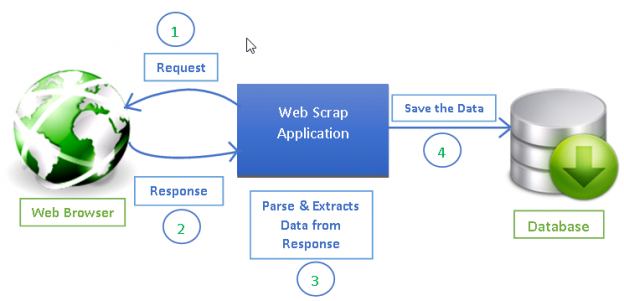
\includegraphics[scale=.5]{custom-web-scraping-624x301.png} 
\end{frame}

\begin{frame}{Barriers to Web Scraping}
\begin{itemize}
\item Not all web pages allows data scraping
\item Captchas block the scraper from proceding further
\item Frequent structural changes made to website
\item IP blocking
\end{itemize}
\end{frame}

\begin{frame}
\frametitle{Implementation Algorithm}
\center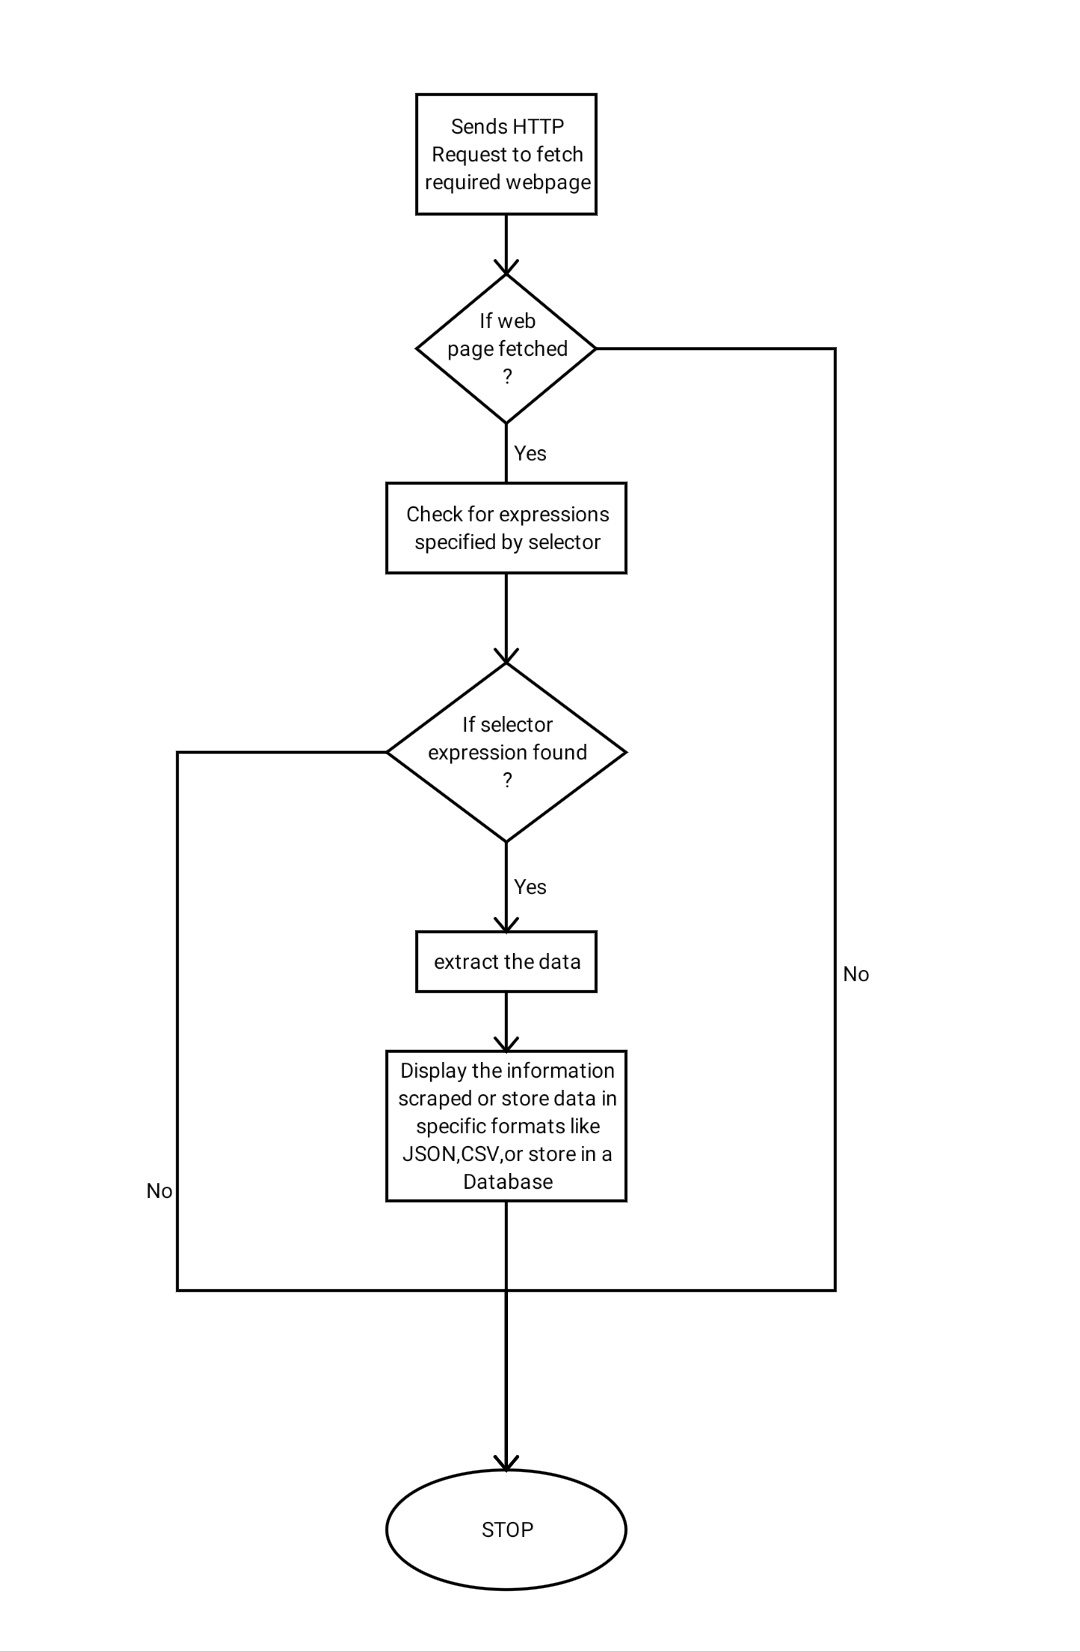
\includegraphics[scale=.12]{IMG_20191017_083215.jpg} 
\end{frame}


\begin{frame}{Spell Checker}
\title{Spell checker}
\begin{enumerate}
\item Aim
\item Introduction
\item Existing Algorithm-1
\item Existing Algorithm-2
\item Proposed Method
\item Proposed Architecture
\item Proposed flowchart
\item Result
\item Conclusion
\end{enumerate}
\end{frame}
\begin{frame}{AIM}
writing a spell checker program to check the correctness of a given document
\end{frame}
\begin{frame}{INTRODUCTION}
We have to create a user program that checks the correctness of a document and makes neccesary changes if needed.Spell-checking features are often embedded in software or services, such as a word processor, email client, electronic dictionary, or search engine. 
\end{frame}
\begin{frame}{EXISTING ALGORITHM PAGE 1-Grammerly}
 Grammarly is an AI powered tool.
 \begin{enumerate}
 
 

\item So it’s basically a computer program or algorithm  which studies and compares your sentence against hundreds of similar ones that are listed in their database.
\item Grammarly, as mentioned earlier, is an AI powered tool that weighs your writing by comparing it against authentic rules and sentence patterns
\item Grammarly’s algorithms flag potential issues in the text and suggest context-specific corrections for grammar, spelling and usage, wordiness, style, punctuation, and even plagiarism using patterns in its database.

\end{enumerate}

\end{frame}
\begin{frame}

\includegraphics[scale=0.5]{grammer.png} 
\end{frame}

\begin{frame}{EXISTING ALGORITHM PAGE 2-GINGER}
 Ginger Software is an Israeli start-up company.
 \begin{enumerate}
 
 \item Ginger Software that has developed language enhancement technology that uses statistical algorithms in conjunction with natural language processing

\item Ginger Software uses patented software algorithms that deal with natural language processing. The company claims that the algorithm allows it to correct the written sentences with relatively high accuracy (eliminating up to 95 percent of writing errors) compared to standard spell checkers. \item Its unique algorithm allows the software to understand the context of the sentence rather than correcting based solely on a word. 
\item The software operates on the logic of sentence context in addition to the memory of a database of words.

\end{enumerate}

\end{frame}
\begin{frame}

\includegraphics[scale=0.5]{ginger.jpeg} 
\end{frame}



\begin{frame}{PROPOSED METHODOLOGY}
To do the User Authentication we use
\begin{enumerate}
\item online Dictionary
\item where we cross check word by word with its counterpart in the dictionary using the first letter as hint.
\end{enumerate}
\end{frame}
\begin{frame}{Proposed algorithm}
 \begin{enumerate}
 
 \item Given document is broken down into words and duplicate words are removed.
\item each word is checked up in the dictionary module and if found is kept or else added to the dictionary if needed or changed by the user if not needed. 
\item the final edition is done by the user and recorrected document is received

\end{enumerate}

\end{frame}

\begin{frame}{FLOW CHART}
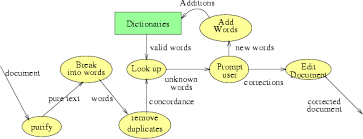
\includegraphics[scale=0.5]{index.png}     
\end{frame}

\begin{frame}{PROPOSED ALGORITHM}
\begin{enumerate}
\item Input URL from user using chatbot
\item run scrapy process using os library 
\item scrap main page of website. Output scraped data to data.json file
\item If user wants to follow to assoiciated links .scrape the follow links too.
\item After scraping, open data.json using file handler.
\item Check for spelling and offensive words in json file
\item If found listed to chat bot as website analysis report
\item end
\end{enumerate}
\end{frame}


\begin{frame}{CONCLUSION}
A bot was created which analyses and monitors a website periodically. It uses help of
three sub programs that is chat bot , spell checker which also checks for offensive
words and a scrapy tool which will scrap the desired web page These sub programs is
later on implemented together to create bot which creates a bot that that checks for the
content of a website given and detects for spelling and offensive words if present in it
and also makes sure to notify of any outside activity.
\end{frame}
\begin{frame}
Initially chat bot was executed and acts as user friendly interface and can be
used to communicate to the bot and later on used to analyze the website which is our
main concern. Th chat bot makes sure to pick up the URL of the website needed and is
given to spell checker to be executed. The chat bot can also generate response on
questions asked by the user based on keyword matching.
\end{frame}

\begin{frame}
The scrapy package used here to scrap data from desired websites. It also
provides an option to follow scrapping to associated links and stores the data into a
document.
\end{frame}
\begin{frame}
Spell checker checks the output file where the scrapped data is stored and
checks for spelling if present and also checks for offensive words If found the words
are returned to chat bot and displayed as the analysis report . It also checks for any
external activities.

\end{frame}


\end{document}
\end{document}